\chapter{Design}

\section{Architecture}
Moving towards architecture (see figure \ref{fig:design_architecture_first}), we first have to separate the whole system into smaller parts.
This way, I identified four main services: 
\begin{itemize}[noitemsep]
    \item \textbf{Auth/User service:} to manage authorization and authentication.
    \item \textbf{Stats service:} to manage all the information related to stats diagram generation. 
    \item \textbf{Test service:} to manage the test creation, e.g. indicate if a reply is correct or not. It should be able to generate the tests from the dataset and get the helper videos to form the tests.
    \item \textbf{Video recognition service:} AI service to validate a video sent by the user. It will label the video.
\end{itemize}

There should be a direct communication between the \textit{Stats service} and the \textit{Test service} because the stats should be created from the data gathered from the tests. \\
Also, there should be communication between the \textit{Video recognition service} and the \textit{Test service} in order to detect if an answer is correct or not. \\

\begin{figure}[H]
    \centering
        \includegraphics[width=\textwidth]{assets/diagrams/services.png}
    \caption{Towards the app's architecture}
    \label{fig:design_architecture_first}
\end{figure}

A refined version of the previous diagram can be seen on figure \ref{fig:design_architecture_last}. 
The user communicates with the app, which is formed by the four subsystems. 
The system has two databases, one for user identification (\textbf{Auth}) and another one for user stats, info about the tests done by them... (\textbf{User stats}). 
Now the \textit{stats service} does not need to communicate with the \textit{test service}, as the stats can be dynamically created. \\

\begin{figure}[H]
    \centering
        \includegraphics[width=\textwidth]{assets/diagrams/architecture.png}
    \caption{App's architecture}
    \label{fig:design_architecture_last}
\end{figure}

\section{Conceptual design}
It is neccessary to identify all the entities of the system to create the database. These entities are shown in an 
E-R (Entity-Relationship) diagram (see figure \ref{fig:design_conceptual}). This way, I identified a new entity: 
\textit{Question}, which is the base component to create a test. The question comes from the \textit{question generator}, which creates the questions using the \textit{video storage service} (which can be an extern service) and the \textit{dataset}.

\begin{figure}[H]
    \centering
        \includegraphics[width=\textwidth]{assets/diagrams/conceptual.png}
    \caption{App's architecture}
    \label{fig:design_conceptual}
\end{figure}

\section{UI design}
\subsection{Low fidelity design}
To validate all the features that the application should have, the navigation, implementation of user stories, design patterns...I created a low-fidelity design. \\

Firstly, I present all the screens and then the navigation between them to show how a user would interact with the application.

\subsubsection{Common}
These are the commons components for the whole application. The \textbf{navbar} and the \textbf{bottom bar}. See figure \ref{fig:design_common}.

The \textbf{navbar} shows basic information about the current user and allows a quick navigation to secondary information about the app.
It allows the navigation to the previous page and contains the title of the current one. The information scheme was designed
using the \textit{3-step rule}.

The \textbf{bottom bar} allow the user to navigate through the main pages of the application. 
It won't be visible in subpages to allow the user to concentrate on the task and save screen space.
\begin{figure}[H]
    \centering
    \includegraphics[width=0.24\textwidth]{assets/screens/Button - User.png}
    \caption{Common components}
    \label{fig:design_common}
\end{figure}

\subsubsection{Authorization}
The next figure \ref{fig:design_screens_auth} shows the initial pages of the application. In order to be used, being logged in is needed, so the user should be firstly registered and then signed in to start a new session.\\

Satisfy: \textit{RF\_1.1} and \textit{RF\_1.2}. \\
\begin{figure}[H]
    \centering
    \begin{subfigure}[T]{0.49\textwidth}
        \centering
        \includegraphics[width=0.48\textwidth]{assets/screens/auth/Login.png}
        \caption{Login screen}
        \label{fig:design_screen_login}
    \end{subfigure}
    \hfill
    \begin{subfigure}[T]{0.49\textwidth}
        \centering
        \includegraphics[width=0.48\textwidth]{assets/screens/auth/Register.png}
        \caption{Register screen}
        \label{fig:design_screen_camera_register}
    \end{subfigure}
       \caption{Authorization screens}
       \label{fig:design_screens_auth}
\end{figure}

\subsubsection{Home}
The home screen (see figure \ref{fig:design_home}) will show the main information a user want to access. This is the recent quizs taken by the user. \\

In addition, I included an \textbf{ad component}, so that the monetization model of the app could be performed via ads. This should be taken into account when the app is going to be launched in production and to create a valid business model.\\

It satifies: \textit{RF\_2.3}. \\
\begin{figure}[H]
    \centering
        \includegraphics[width=0.24\textwidth]{assets/screens/Home.png}
    \caption{Home screen}
    \label{fig:design_home}
\end{figure}

\subsubsection{Quiz}
These are the common components/screens for the quizzes: \\

\begin{itemize}[noitemsep]
    \item \textbf{Result screen:} the user can see how they performed doing the current quiz. See figure \ref{fig:design_screen_result}.
    \item \textbf{Selecting difficulty screen:} the user will be able to customize a quiz, selecting the \textbf{difficulty} and the \textbf{number of questions} of a test. See figure \ref{fig:design_screen_select_dif}.
    \item \textbf{Selecting quiz's type screen:} the user will be able to select the \textbf{test type} before starting a new one. See figure \ref{fig:design_screen_select_quiz}.
\end{itemize}

\begin{figure}[H]
    \centering
    \begin{subfigure}[T]{0.32\textwidth}
        \centering
        \includegraphics[width=0.72\textwidth]{assets/screens/quiz/common/Quiz - Result.png}
        \caption{Result of a test}
        \label{fig:design_screen_result}
    \end{subfigure}
    \hfill
    \begin{subfigure}[T]{0.32\textwidth}
        \centering
        \includegraphics[width=0.72\textwidth]{assets/screens/quiz/common/Select difficulty.png}
        \caption{Select difficulty of a test}
        \label{fig:design_screen_select_dif}
    \end{subfigure}
    \hfill
    \begin{subfigure}[T]{0.32\textwidth}
        \centering
        \includegraphics[width=0.72\textwidth]{assets/screens/quiz/common/Select quiz.png}
        \caption{Select type of test}
        \label{fig:design_screen_select_quiz}
    \end{subfigure}
       \caption{Common screens for all tests}
       \label{fig:design_test_common}
\end{figure}

The components of the quizzes depending on the test type are (see figure \ref{fig:design_test_screen}):
\begin{itemize}[noitemsep]
    \item \textbf{Mimic:} the question is composed by the word to sign and a help video. The user should sign that word and can watch the help video to imitate it.
    \item \textbf{Option video to word:} the question is composed by a video representing a sign and 4 options (words). The user should select the word matching the video.
    \item \textbf{Option word to video:} the question is composed by a word and 4 videos representing signs. The user should select the video corresponding to the word.
    \item \textbf{QA:} the question is composed by just the word to sign. The user should sign the word.
\end{itemize}
They have in common a button to \textbf{skip} a question and a component with information related to the current quiz (test type, number of questions and current question). \\

\begin{figure}[H]
    \centering
    \begin{subfigure}[T]{0.24\textwidth}
        \centering
        \includegraphics[width=\textwidth]{assets/screens/quiz/Quiz - Mimic.png}
        \caption{Mimic}
        \label{fig:design_screen_mimic}
    \end{subfigure}
    \hfill
    \begin{subfigure}[T]{0.24\textwidth}
        \centering
        \includegraphics[width=\textwidth]{assets/screens/quiz/Quiz - Option 1.png}
        \caption{Option video to word}
        \label{fig:design_screen_mimic}
    \end{subfigure}
    \hfill
    \begin{subfigure}[T]{0.24\textwidth}
        \centering
        \includegraphics[width=\textwidth]{assets/screens/quiz/Quiz - Option 2.png}
        \caption{Option word to video}
        \label{fig:design_screen_mimic}
    \end{subfigure}
    \begin{subfigure}[T]{0.24\textwidth}
        \centering
        \includegraphics[width=\textwidth]{assets/screens/quiz/Quiz - Q_A.png}
        \caption{QA}
        \label{fig:design_screen_mimic}
    \end{subfigure}
       \caption{Tests' screens}
       \label{fig:design_test_screen}
\end{figure}

These screens represent how a user could answer a question if they are asked to send a video. They could select a video from the gallery or record themselves signing the word (see figure \ref{fig:design_screen_camera}), and send the video to the application or record it again (see figure \ref{fig:design_screen_camera_send}). \\
\begin{figure}[H]
    \centering
    \begin{subfigure}[T]{0.49\textwidth}
        \centering
        \includegraphics[width=0.48\textwidth]{assets/screens/quiz/quiz-camera/Quiz - Camera.png}
        \caption{Camera}
        \label{fig:design_screen_camera}
    \end{subfigure}
    \hfill
    \begin{subfigure}[T]{0.49\textwidth}
        \centering
        \includegraphics[width=0.48\textwidth]{assets/screens/quiz/quiz-camera/Quiz - Camera send.png}
        \caption{Send photo}
        \label{fig:design_screen_camera_send}
    \end{subfigure}
       \caption{Reply to test using the camera}
       \label{fig:design_camera}
\end{figure}

\subsubsection{Stats}
The first screen (see figure \ref{fig:design_screen_stats_1}) represents the most basic information: the \textbf{percent of learnt words} and the \textbf{use of the app} (in the calendar a user can see the days they have used the application starting a new quiz). They can also consult the maximum number of days they have used the application in a row and the current streak. \\

The second screen (see figure \ref{fig:design_screen_stats_2}) shows more information about the app to the user: \textbf{time spent} in the app and \textbf{new words learnt}, as well as the \textbf{success rate}. The users can filter the stats by date (and/or) by difficulty. \\

The third screen (see figure \ref{fig:design_screen_stats_3}) show another way of representing the stats, in a more detailed way using graphs. \\

Satisfy: \textit{RF\_3.1} and \textit{RF\_3.2}. \\
\begin{figure}[H]
    \centering
    \begin{subfigure}[T]{0.32\textwidth}
        \centering
        \includegraphics[width=0.72\textwidth]{assets/screens/stats/Stats - 1.png}
        \caption{Stats: page 1}
        \label{fig:design_screen_stats_1}
    \end{subfigure}
    \hfill
    \begin{subfigure}[T]{0.32\textwidth}
        \centering
        \includegraphics[width=0.72\textwidth]{assets/screens/stats/Stats - 2.png}
        \caption{Stats: page 2}
        \label{fig:design_screen_stats_2}
    \end{subfigure}
    \hfill
    \begin{subfigure}[T]{0.32\textwidth}
        \centering
        \includegraphics[width=0.72\textwidth]{assets/screens/stats/Stats - 3.png}
        \caption{Stats' detail}
        \label{fig:design_screen_stats_3}
    \end{subfigure}
       \caption{Stats' screens}
       \label{fig:design_screen_stats}
\end{figure}

\subsubsection{User}
This screen (see figure \ref{fig:design_user}) allows the user to customize the application and change their personal information. \\
\begin{figure}[H]
    \centering
        \includegraphics[width=0.24\textwidth]{assets/screens/User.png}
    \caption{User screen}
    \label{fig:design_user}
\end{figure}

\subsubsection{Navigation}
In the figure \ref{fig:design_lofi} we can see how a user would interact with every screen and the navigation between all of them.

Firstly, there is a first layer that the user has to pass, which is the auth layer. In order to use the rest of the application (private routes), the user
must sign in the application.

Secondly, there is a row containing the main screens of the application. Using the \textbf{bottom bar} the user is able to move from one to another.

Finally, we see the subpages of the application.
I represented a use case: create a test and do it. The user starts the quiz selecting the difficulty, number of questions and type of quiz. Then the user replies to the questions of the quiz itself and then the user sees the quiz result.

\begin{figure}[H]
    \centering
        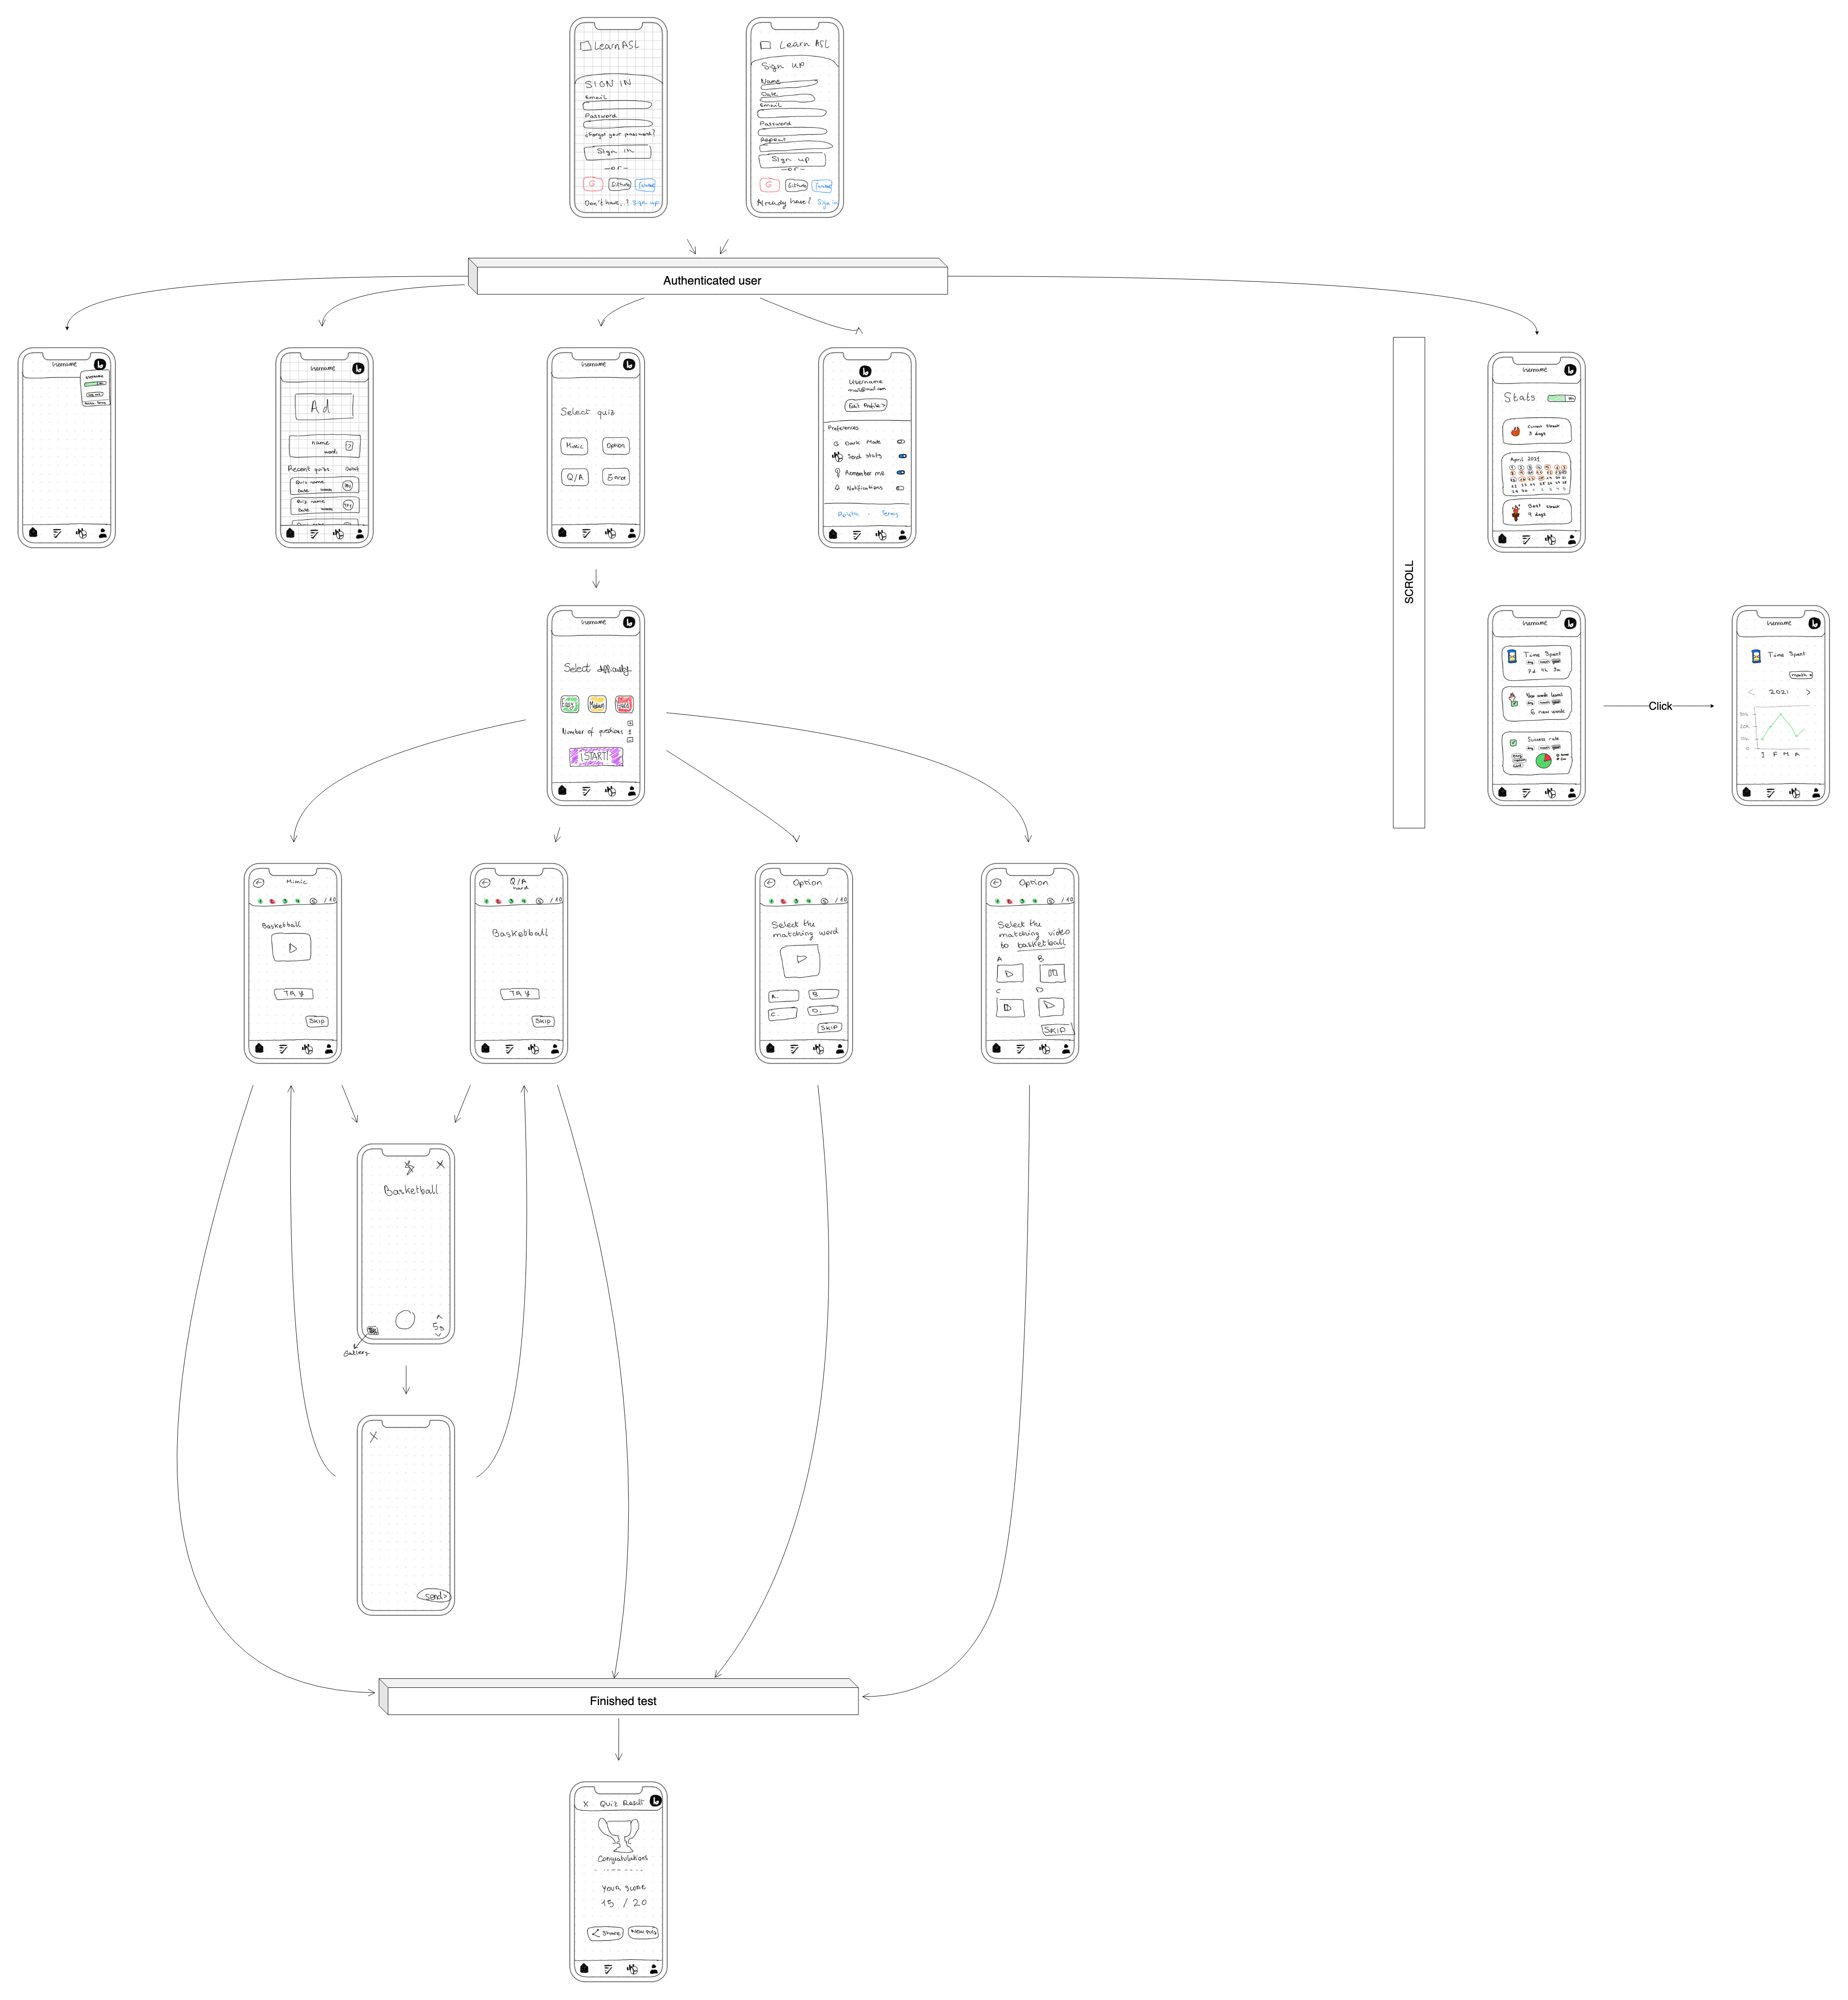
\includegraphics[width=\textwidth]{assets/lofi.png}
    \caption{Low-fidelity design}
    \label{fig:design_lofi}
\end{figure}

